\chapter{Algorithm}

First of all, we need to answer two questions:

\begin{enumerate}
  \item How the subgraph density should be measured?
  \item What is <<the most of the selected vertices>>?
\end{enumerate}

To compare two subgraphs obtained by different algorithms we will use edge density and the size of the resulting subgraph: $density(G) = \frac{2 \cdot |E(G)|}{|V(G)| \cdot (|V(G)| - 1)}$, $size(G) = |V(G)|$. Really, if the number of edges in obtained subgraph is quite big, we can assume that it is dense. However at the same time it should have the smallest possible size. What is <<the most of the selected vertices>> will be discussed a bit later.

\section{Idea of the algorithm}

Because there are quite few algorithms that solves exactly our problem, we have two ways: to come up with absolutely new idea and algorithm or to take an existing idea and try to improve it or to make it work on our problem instead of common \textit{CSP} with all query vertices needed to be in resulting subgraph. Starting from now we will use \textit{CSP} abbreviation for community search problem, where all query vertices should be presented in the resulting subgraph and \textit{NCSP} for noisy version of the problem, what we need only most of the query vertices in the answer.

Absolutely new algorithm may look like this: we can bruteforce the set of vertices which will be noise, then find dense subgraph that contains all query vertices except bruteforced ones using one of the described in first chapter solutions and we're done. This solution will obviously return the most optimal answer, but it works too slow, the complexity of this solution is not polynomial. So, we won't use this method and will try to come up with something else.

The easier way is to take some existing algorithm for \textit{CSP} and transform it for \textit{NCSP}. Really, it is proved that such algorithm works good and is one of the best for now, so we have a lot of chances to beat all current \textit{NCSP} solutions in that case. Here we go: let's take algorithm Barbieri et al. \cite{Barbieri15} for finding $k$-core with maximal $k$ and minimal size and try to optimize it and change so that is will solve \textit{NCSP}. One more note that makes us more assured about this idea is two articles~--- Bogdanov et al. \cite{Bogdanov13} and Cui et al. \cite{Cui14} which showed that maximization of the minimal degree in subgraph is very effective for finding the optimal community, so our idea absolutely may take place.

The idea of Barbieri et al. algorithm \cite{Barbieri15} is in finding in graph $G$ \textit{k-core} with the maximal $k$ and among all such solutions, we want to find the one with the minimal number of vertices in it. In their work, authors show that it is a NP-hard problem, so we need to use some heuristics to solve it. The idea of algorithm is based on one interesting fact, which we're going to use in our work as well: consider the core decomposition of graph $G$: $C = \{C_k\}_{k=1}^{k=k^*}$. Now let's find such maximal $k'$ that all vertices from query are lying in the same component of $H^* \in C_{k'}$. The fact is that all solutions for \textit{CSP} are lying in this component $H^*$. More formally: $k' = \max\{k | \exists H_i\mbox{~--- connected component } C_{k'}\mbox{, such that } \forall v \in Q: v \in H_i\}$. The found \textit{k-core} we will denote as $C_Q^*$ and the component which contains all query vertices~--- $H^*$. We need to note two things here: first~--- this statement helps us to decrease the size of the initial graph without loosing solutions and second~--- this statement is true even for \textit{NCSP}, because if $H^*$ contains all optimal subgraphs with all query vertices, it contains all optimal subgraphs containing only a subset of query vertices as well. It is possible that the resulting subgraph will be a \textit{k-core} with bigger $k$ than $H^*$ have, but nothing prevent us from starting our algorithm from $H^*$.

Let's explain the final idea of our algorithm: by given social network $G$ and the selected vertices $Q$, we will find \textit{k-core} $C_Q^*$ and its connected component $H^*$ that contains all optimal solutions for \textit{NCSP}. $H^*$ is actually one of the candidates for the answer, because it contains all vertices from $Q$, but it's too large and we want to make it smaller (also, this subgraph contains all query vertices, i.e. the noise as well). So, after we found $H^*$, we are going to apply some heuristics that will allow to decrease the size of $H^*$ without loosing the condition on minimal vertex degree (i.e. \textit{k-core} invariant) and therefore not making the answer worse.

\section{Step-by-step algorithm}

In this section we will describe the whole algorithm. Actually, we can divide the algorithm into two phases:

\begin{enumerate}
  \item Find $C_Q^*$ and $H^*$;
  \item Decrease size of $H^*$ without loosing the \textit{k-core} property. 
\end{enumerate}

Actually, in future we will split the second phase into several more, but let's talk about it later. Now we will try to sort out with each phase separately.

\subsection{Phase 1. Finding $C_Q^*$ and $H^*$}

$C_Q^*$ and $H^*$ finding phase will be taken from Barbieri et al. article \cite{Barbieri15} as well as their idea of minimization of \textit{k-core}. It's easy to see that actually core decomposition doesn't depend on the query, so it's not necessary to build it each time. But unfortunately saving it in RAM before all the queries is not a good idea as well, because it's size may be too big. That's why we're going to do a pre-calculation which will build a core decomposition once, compress it and save on disk. It will be a so-called index which will allow us to find $C_Q^*$ and $H^*$ much faster for each query.

In index of our core decomposition $C = \{C_k\}_{k = 1}^{k = k^*}$ we will store the following information:

\begin{enumerate}
  \item Core indices for all vertices $c(v) = \max\{k \in [0..k^*] | v \in C_k \}$;
  \item For each \textit{k-core} $C_k$ we will store the set of its components $C_k = \{H_i\}$.
\end{enumerate}

The following picture illustrates the above statements~\ref{index-construct}:

\begin{figure}[!h]
\caption{Index construction}\label{index-construct}
\centering
  \begin{center}
    \makebox[\textwidth]{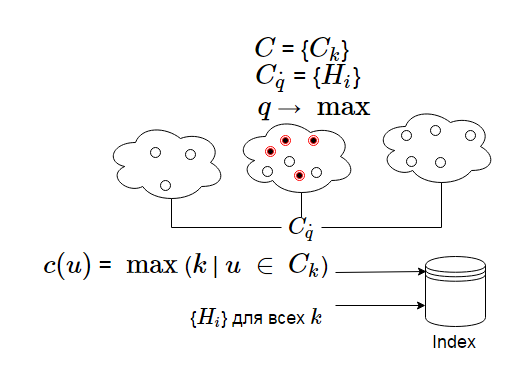
\includegraphics[scale=0.8]{pictures/index.png}}
  \end{center}
\end{figure}
\FloatBarrier

We also need to take a small note that some neighboring \textit{k-core}s are equal: $C_k = C_{k + 1}$. There is no need to store them twice, so we will store all duplicating neighboring \textit{k-core}s only once. For now it doesn't look like a very good optimization, but actually on the real datasets the number of different \textit{k-core}s may be even several orders less, so this optimization makes sense. We will also use variable $h$ in future~--- it means the number of different \textit{k-core}s in our core decomposition, i.e. the number of \textit{k-core}s which we're going to store in our index.

We will store code indices and sets of connected components in the appropriate data structures (hash tables). It will allow us to access the following object in $O(1)$ complexity:
\begin{itemize}
  \item $c(v)$;
  \item all components of the fixed \textit{k-core};
  \item a component of the fixes \textit{k-core} where the given vertex $v$ is located.
\end{itemize}

But actually we haven't said yet how to build this index. Actually it's quite simple: let's firstly build the set of components for $C_{k^*}$, after that all other \textit{k-core}s will be built in the following way: if \textit{k-core}s for $k^*, k^*-1, \ldots, k$ are already built, then to build \textit{$(k - 1)$-core} we will add all vertices from $C_{k - 1} \setminus C_k$ one by one and edges incident to them (according to the property that $C_{k - 1} \supseteq C_k$, it's enough) and then we will update connected components which according to the new vertices can union in new, bigger components.

This phase takes $O(h \cdot |V(G)| + |E(G)|)$ time or simply $O(hn + m)$, where $h$ as you can remember is the number of different \textit{k-core} in $G$. However this asymptotic won't be taken into the final consideration because for each graph this computation is taken only once (so we can wait if needed) and then the built index is used for finding $C_Q^*$ and $H^*$ for each query.

So, how can we find $C_Q^*$ and $H^*$ by our built index? Actually, it's very simple. Because $C_1 \supseteq C_2 \ldots \supseteq C_{k^*}$, to find \textit{k-core} with maximal order that contains all query vertices from $Q$ in its one component, we can use binary search by the \textit{k-core} order. To check if for some fixed $k$, $C_k$ contains all vertices of $Q$ in its one component, we will take for each vertex from $Q$ information about the component it is lying in (using the index, we can do it in $O(1)$ time) and then check that all these numbers are equal. So, the check for each binary search step will take $O(|Q|)$ time.

Summing up everything above, we see that the step of finding $C_Q^*$ and $H^*$ takes $O(|Q| \cdot \log(h))$.

\subsection{Phase 2. Decreasing $H^*$ size}

After finding $C_Q^*$ and its connected component $H^*$ that contains all vertices from $Q$ as we mentioned earlier it's easy to see that $H^*$ is the answer for our problem, because all its vertex degrees are at least $k$ and $k$ is the maximal possible (according to $H^*$ construction). However, we still have one more condition to be true~--- the resulting graph should have the minimal possible size, now it's obviously not true. This is what we're going to fix in this and the next phases. In this phase we are going to remove noise from $H^*$, i.e. to select its subgraph which contains most of the query vertices (except the noise).

Let's remind that the problem of finding minimal by size \textit{k-core}~--- NP-complete. Which heuristics can we use? The first idea which comes to mind is to delete weakly connected vertices or subgraph from $H^*$, therefore making its size smaller. However, because all vertices degrees are at least $k$, it may be hard to understand which vertices are weakly connected and which are not. Also, it's not obvious how to understand which subgraphs can be deleted without loosing the condition for minimal vertex degree.

We've chosen a reverse approach~--- adding vertices. We will build the final subgraph $H_{min}$ in the following way: let's take all query vertices $Q$ and delete all other vertices and edges. After that we will add other vertices one by one with some priority, making our subgraph $H_{min}$ larger and more connected. At each moment, when the current subgraph satisfies the answer for our problem (i.e. the component of the current subgraph $H_{min}$ with the maximal number of query vertices in it, contains <<the most of the query vertices>> and it is also <<dense enough>>), we will update the final answer. It's obvious that the process is finite~--- the number of vertices in the current subgraph is growing and we won't obtain the subgraph larger than $H^*$. However we face three global questions:

\begin{enumerate}
  \item What is the priority for adding vertices to the current subgraph?
  \item When do we need to update the answer (i.e. what is <<the most vertices from $Q$>>, and what is <<component is dense enough>>)?
  \item When do we need to stop adding vertices?
\end{enumerate}

\textbf{a. What is the priority for adding new vertex?}

There are tons of priority options. However let's think, what metrics are important for us. Firstly, we want vertices that form a community (i.e. the set of query vertices without the noise) to be united into one connected component as soon as possible and began to increase this component density. So, as the first priority we will take the number of components which the newly added vertex unite. I.e., $p_1(v) = |A'| - |A|$, where $A$ is the set of components before adding $v$ and $A'$ is the set after adding it. However after adding the new vertex in many cases the number of components won't change. What do we need to do in this case? Because vertex degrees in the final subgraph are also important for us, let's emphasize attention on it. When adding vertex $v$, degrees of its neighbors which are already contained in the current subgraph, are increased by $1$. We want to maximize this count. However, we also need to take into account the recently added vertex and its degree. So, let's make the following second priority: $p_2(v) = |N_{H_{min}}(v) \cap \{v \in V(H_{min}) | deg(v) < \mu(H^*)\}| - \max(0, \mu(H^*) - |N_{H_{min}}(v)|)$, where $N_{H_{min}}(v)$ is the set of vertices from $H_{min}$ which are connected with $v$ by edge. In other words, we take the number of neighbors of vertex $v$ from $H_{min}$ for which degree is less than needed $\mu(H^*)$ for now with plus sign and the number of edges which is needed for the recently added vertex to have degree $\mu(H^*)$ with minus sign.

\textbf{b. What is <<the most of the vertices from Q>>, what does <<the component is dense enough>> mean?}

We will say that subgraph $H \subset G$ contains for most of the vertices from $Q$ if the number of query vertices in it is at least $\alpha(|Q|) \cdot |Q|$. $\alpha(|Q|) \in (0, 1]$ or just $\alpha$ is some coefficient which depends on the number of query vertices. But what $\alpha$ should be equal to? From one side we want <<the most of the vertices>> to be really the most part of them, so we will assume that there is less than $\frac{|Q|}{2}$ noise vertices in the query (i.e. $\alpha \ge 0.5$). From the other hand, even $\frac{|Q|}{2}$ noise vertices is too much in most cases.

We are also interested in what <<the component is dense enough>> means. We will say that the component is dense enough if it contains enough edges (it obviously means that its dense is quite high). To select the bound of the edges count we tried several functions, and the most optimal one turned out to be the following: $|E(H_{min})| \ge (V(H_{min}) - |Q|) \cdot \mu(H^*) + \beta(|Q|) \cdot |Q|)$, i.e. for all query vertices we take their degree equal to $\beta$ (one more parameter) and for other ones degree should be at least $\mu(H^*)$ (actually if there is some noise in the query, degree should be even higher, however, if there is no noise, the previous statement is true).

To choose optimal values for parameters $\alpha$ and $\beta$ given the fixed $|Q|$ we decided to make some experiments (they we made on the same data as all other experiments described in chapter $3$). Results of the experiments are shown in the table below ($k$ is the order of \textit{k-core}, i.e. $k = \mu(H^*)$).

\begin{table}[!h]
\centering
\caption{Optimal values for $\alpha$ and $\beta$ for different $|Q|$}\label{parameters-research}
  \begin{tabular}{| l | l | p{1cm} |}
  \hline
  $|Q|$ & $\alpha$ & $\beta$ \\\hline
  2   & 1      & 1        \\\hline
  3   & 2 / 3  & 1        \\\hline
  4   & 1 / 2  & 1        \\\hline
  5   & 3 / 5  & 2        \\\hline
  6   & 2 / 3  & 2        \\\hline
  7   & 4 / 7  & 3        \\\hline
  8   & 3 / 4  & 3        \\\hline
  > 8 & 7 / 10 & 4        \\\hline
  \end{tabular}
\end{table}
\FloatBarrier

\textbf{c. When the algorithm should be stopped?}

It's simple to understand that the algorithm can be stopped when all vertices from $H^*$ are added. However, because the size of $H^*$ may be quite big, it's not the optimal solution~--- when our current subgraph became connected, it will contain all query vertices and thus all the noise, while our task is to avoid noise in the result subgraph. So let's stop our algorithm when our current subgraph became connected, we won't loose any answers in that case.

\begin{figure}[!h]
\caption{Example of phase $2$ work}\label{phase2-example}
\centering
  \begin{center}
    \makebox[\textwidth]{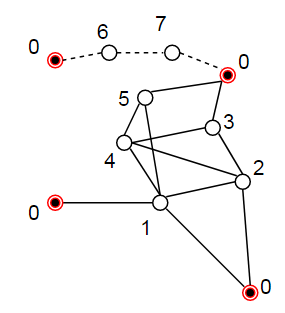
\includegraphics[scale=1.2]{pictures/phase2.png}}
  \end{center}
\end{figure}

Let's assume that $H^*$ looks like at the picture~\ref{phase2-example}. Query vertices are marked red, we're taking them at the first step. After that we will add vertices one by one, as it is shown on the picture: firstly we add vertex $1$, because it unites two components, then $2$ because it has the maximal second priority, etc. Our algorithm finishes when $H_{min}$ becomes connected, in that case it will happen when all edges will be added. However, the optimal subgraph will be the one without the dotted edges, because it will be more dense. And as we can see the vertex that was not added is an obvious noise, so we shouldn't add it to the result subgraph.

\subsection{Phase 3. Restoring the condition for vertex degrees}

After phase $2$ is completed, we have a subgraph $H_{min}^*$. This subgraph can be returned as the answer, but of course as we just saw on the picture~\ref{phase2-example}, $H_{min}^*$ can be far away from the optimal answer. Why? We were adding vertices one by one with, as it seemed, optimal priority. Actually, because we focus on adding vertices that unite our current components the best and take vertex degrees into account only as the second priority, the obtained subgraph can be non-optimal. That's why we need to do something with $H_{min}^*$ to satisfy the condition for vertex degrees.

You may now think that phase $2$ was redandunt, because we had the \textit{k-core} which was densely connected and we obtained the subgraph which is not \textit{k-core} and thus is not densely connected. That's not true, because the initial \textit{k-core} contained all query vertices and new subgraph doesn't contain query noise. Also, as you will see, we will apply some heuristics and new subgraph $H_{min}^*$ will become a dense \textit{k-core} of bigger order.

To begin with, let's remove weakly connected vertices. Because our new subgraph $H_{min}^*$ is not a \textit{k-core}, we can suggest logical conditions for that. Let's remember parameter $\beta$ which we introduced to be responsible for the minimal query vertex degrees. Let's remove all query vertices that have degree less than $\beta$, i.e. which doesn't follow our invariant. After deletion, let's run phase $1$ one more time on the left query vertices. Actually, we don't need to run the whole phase $1$, we only need to find the new value $k^{opt}$~--- the maximal order of \textit{k-core} in which all remaining query vertices lie in the same component.

Now we will do the main step of the final phase. Its idea is in the following: we will take all remaining query vertices and find the minimal number of non-query vertices that connect them. In other words, taking the remaining subset of query vertices $Q' \subseteq Q$ we want to find such set of vertices $V_{opt} \subseteq V(H_{min}^*) \setminus Q'$ of minimal size so that $G[V_{opt} \cup Q']$ is connected (to remind, $G[V]$ is a subgraph originated by the set of vertices $V$). It will give us a <<skeleton>> of subgraph $H_{min}^*$ which we will build up almost the same way as we were doing in phase $2$.

The problem that we have described above is a \textit{Steiner task}. The original version of Steiner task sounds as follows: given a weighted graph $G$ and a subset of selected vertices $Q$ in it, you need to find a minimal spanning tree on the selected vertices. It's quite interesting that for $|Q| = 2$ the task is just to find the minimal path between two vertices, if $|Q| = |V(G)|$, the task is just to find the minimal spanning tree, and in all other cases the task is NP-hard. You can mention that in our case graph is unweighted, but actually Steiner task remains NP-hard even on unweighted graphs. Steiner task have been investigated many years ago, and Kou et al. \cite{Kou81} gave us an optimal algoriths for solving it with approximation $2 - \frac{2}{|Q|}$ and proof that it's impossible to solve it better in polynomial time. We will take this solution and apply it to our task.

After finding the needed <<skeleton>>, we will apply slighly modified phase $2$ to it. First, skeleton is already connected and we don't need priority for uniting the components. Second, we want to guarantee the density of the final subgraph, so we need to modify condition a little bit:

\begin{enumerate}
  \item We will add new vertices only by second priority;
  \item We will stop only when the minimal vertex degree is at least $k^{opt}$, because we know that it's possible to build \textit{$k^{opt}$-core} on the remaning query vertices;
  \item We won't update the answer during these iterations, we will take the final subgraph as the answer.
\end{enumerate}

After changing the phase $2$ as described above, we apply it on $H_{min}^*$ with deleted weakly connected query vertices and get the final answer to the task.

\begin{figure}[!h]
\caption{Phase $3$ example}\label{phase3-example}
\centering
  \begin{center}
    \makebox[\textwidth]{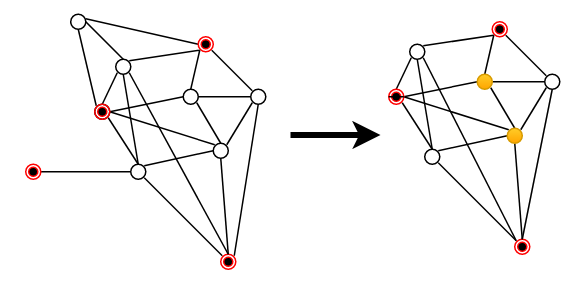
\includegraphics[scale=1.0]{pictures/phase3.png}}
  \end{center}
\end{figure}

The work of this phase is presented on picture~\ref{phase3-example} where subgraph $H_{min}^*$ (3-core) is places on the left and the final subgraph obtained after phase $3$ is placed on the right. First, we remove weakly connected query vertex and then found two yellow vertices which along with remaining query vertices give as a skeleton of $5$ vertices. After that we apply modified phase $2$ on the skeleton and obtain the final subgraph. As you can see, it is smaller and more dense than the first one~--- it is even 4-core when the previous was only 3-core.
